\section{Architecture}
The platform should be able to accomodate the ability for teachers to create a syllabus that includes sessions, exercises and test cases for the exercises. Additionally, the platform should have the ability for students to do the exercises that the teacher has provided. 
The platform should be a web application, consisting of a user-interface, business logic to handle requests, authentication and compilation of the code as well as a database to persist relevant data.
Based on these requirements we have created the architecture seen in figure \ref{fig:Architecture}.

\begin{figure}[H]
	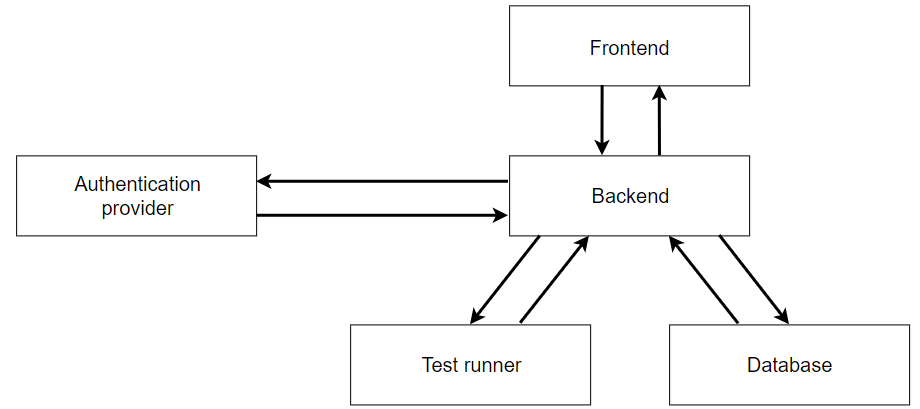
\includegraphics[scale=0.6]{Architecture.PNG}
	\centering
	\caption{The architecture for the web application}
	\label{fig:Architecture}
\end{figure}

In the following sections we will describe the general structure of each component and its responsibility.

\subsubsection{Frontend}
The frontend is the user facing component of our web application. The frontend is designed such that the user-interface and the functionality on the frontend is dependent on the role of the user. 
For example if the signed in user has a student role, the user will be able to see and complete exercises, where if the user has a role of teacher, they will have access to more functionality such as creating a syllabus or exercise.

Therefore the responsibility of the frontend can be split into two categories: 
\begin{itemize}
    \item \textbf{Teacher}-based responsibilities and,
    \item \textbf{Student}-based responsibilities.
\end{itemize}

\subsubsection*{Teacher-based responsibilities}
If the signed in user is a teacher the frontend provides the user the ability to create syllabi, sessions, exercises and test cases for the given exercise, as well as they ability to complete exercises. The latter functionality was included to allow teachers to try out the exercises and ensure that the test cases behave as expected before releasing the exercise to the students. Additionally, the teacher will also have access to a dashbord that shows which students have completed which exercises for a given session, in order to track progress and potential pain points.

\subsubsection*{Student-based responsibilities}
Conversely, if the signed in user is a student, the fronted provides the user the ability to view syllabi, sessions and exercises as well as the ability to attempt exercises. A student will also have access to an overview showing which courses are available to the student and which exercises have been completed. 

\vspace{0.5cm}

Regardless of the roles of the user the frontend has the ability to persist data and execute code through communication with the backend system.

\subsection{Back-end system}
The backend system has several responsibilities including routing, data retrieval and updates, execution of code tests and communication with the authentication provider. The backend provides all the functionality that is essential to our web application and operates as a traditional server in a client-server architechture. 

\subsection{Database}
In order persist data the backend retrieves and updates data in the database component depicted in figure \ref{fig:Architecture}. This is done through create, read, update and delete operations. 
The backend then queries the database and returns the relevant data. 

The database component is implemented as a Postgres database which is a regular relational database. The entities and their relationships contained within the database is shown in figure \ref{fig:Database}. In the figure each box represents an entity-set and attributes for the entities. A diamond represent a relationship between two or more entity-sets.

A dotted line connecting an entity-set to a relationship represent a partial participation of the connected entities and the other participants in the relationship. This means that an entity can exist in the database without participating in the relationship.
A full line connecting an entity-set to a relationship represents total participation of the entity-set symbolising that an entity must participate in the relationship. 
This means that an entity cannot exist in the database without participating in the relationship.
The numbers and letters at the beginning of each relationship line represents the cardinality. A \textit{number} between a relationship and an entity-set represents the number of times an entity can participate in the relationship. Similarily, an \textit{N} represents that entities can participate $0$ or more times.

\begin{figure}[H]
	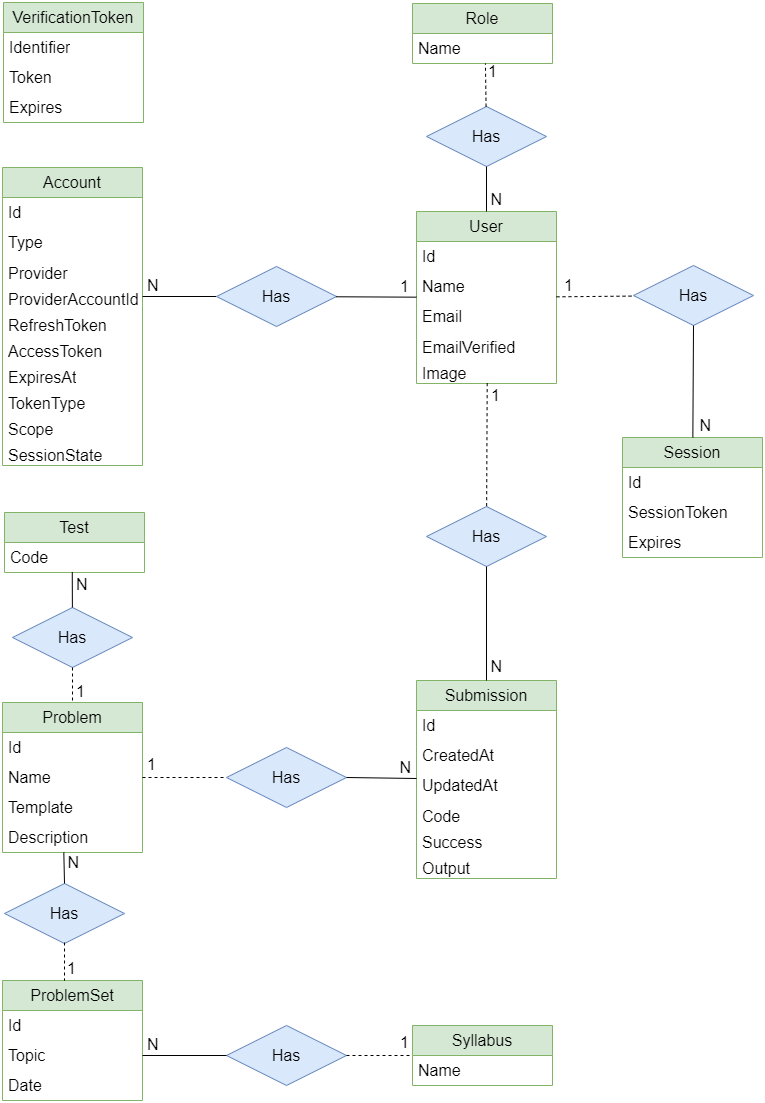
\includegraphics[scale=0.4]{Database.png}
	\centering
	\caption{Entity relationship diagram of the database}
	\label{fig:Database}
\end{figure}


\subsubsection{Test runner}
As mentioned previously the platform needs to be able to run code on back-end and verify whether this code is syntactically correct and safisfies the teacher defined tests.
The component is structured as a layered architecture where each layer is a module and each module has a single responsibility with no global state and full encapsulation.
This means that each component can depend only on components on a lower or same level. For example if component A is on a lower level than component B, component A cannot use component B.
This makes the architecture decoupled and therefore it is easy to add, replace and modify components.

The component structure can be seen in figure \ref{fig:TestRunner}

\begin{figure}[H]
	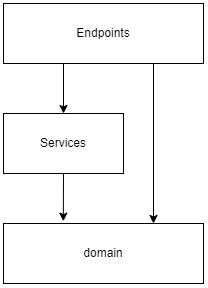
\includegraphics[scale=0.4]{TestRunner.jpg}
	\centering
	\caption{The test runner component architecture}
	\label{fig:TestRunner}
\end{figure}

\subsection{Authentication provider}


